\subsection{The gluon PDF (a.k.a Suppressing the QUark in the Region of RElative Large-$x$)}
(Simone, Gregory, Eric)

Parton Distribution Functions (PDFs) describe the non-perturbative dynamics of quarks and gluons in the protons that take part in high-energy collisions. Therefore, they are a key ingredient for every theoretical prediction that aims to describe particle interactions at high-energy colliders such as the LHC. As a consequence, their precise determination is of utmost importance for LHC phenomenology. 
%
The non-perturbative nature of PDFs hampers their determination from first principles.
%
However, for inclusive enough processes, they are universal, i.e.\, up to power corrections, they do not depend on the particular process, and they can be determined by fitting data from previous experiments. Moreover, although they are themselves non-perturbative objects, their dependence on the energy is governed by the DGLAP equation and the evolution kernels can be computed as a power expansion in the strong coupling. This implies that data collected at past experiments, at different energies, can be used to constrain PDFs. 

Traditionally, the main source of uncertainties assigned to the determination of PDFs arises from the experimental error of the data that enter the fit.~\footnote{Very recently, the inclusion of theory uncertainties in PDF determination has also been achieved~\cite{Harland-Lang:2018bxd,AbdulKhalek:2019ihb,AbdulKhalek:2019bux}} In extreme regions of phase-space, for instance at small- or large-$x$, the experimental uncertainties typically deteriorate and one has to face a reduced number of data points. This is reflected in PDFs which are largely unconstrained in these regions. 
%
For instance, the large PDF uncertainty in the $x\to 1$ region has a negative impact on searches for new and heavy states.
%
 Although this will probably not wash out a potential discovery, it will definitely obscure the nature and the properties of the new state, such as its mass and its couplings. 
%
The way to reduce this PDF uncertainty is to include in the fit data at larger $x$. This cause interesting theoretical issues, because fixed-order perturbation theory becomes less reliable and one should supplement theoretical predictions with threshold resummation, as studied for instance in~\cite{Corcella:2005us,Sato:2013wea,Westmark:2013vea,Bonvini:2015ira,Accardi:2014qda}.


In this study, we focus on the gluon PDF in the region of relatively large longitudinal momentum fraction, $x\sim 10^{-1}$ \sm{check}. The datasets that mostly constrain the gluon in this region are the inclusive jet spectra, in the region of the jet transverse momentum above 1~TeV and the production of top quark pairs. From a theoretical point of view, both processes are known to very high accuracy, i.e. next-to-next-to-leading order (NNLO)~\cite{}. Phenomenologically, the two processes have pros and cons. Inclusive jet production features high statistics across a wide kinematical range and, consequently, even in the high $p_t$ region we are interested the experimental uncertainties do not exceed 10\%. However, because we are measuring inclusive jets we cannot distinguish the flavour content and the cross section is dominated by quark-quark scattering, which bear little information about the gluon PDF. 
%
On the other hand, at LHC energies, top pair production is dominated by gluon fusion and therefore offers a direct probe of the gluon luminosity. In this case, however, we pay a much higher price in terms of experimental uncertainties, essentially because we run out of statistics of values of the top transverse momentum much smaller than for inclusive jets. 
%
Ideally, we would like to exploit the vast jet samples collected by the LHC experiments to tease out more information about the gluon PDF. We immediately realise that one way of achieving this scope would be to supplement the inclusive jet $p_t$ spectrum with some information about the jet flavour. That is, we are going to explore the possibility of using the \emph{inclusive gluon-jet $p_t$} spectrum to extract parton densities, rather than its flavour-blind version.  Properly defining quark jets versus gluon jets is a very active area of jet substructure~\cite{} and indeed it was one of the focus of a past edition of the Les Houches proceedings~\cite{Badger:2016bpw} (see also the follow-up study~\cite{Gras:2017jty}). 


\begin{figure}
\begin{center}
\includegraphics[width=0.49\textwidth, page=9]{figs/fractions.pdf} \hfill
\includegraphics[width=0.49\textwidth, page=10]{figs/fractions.pdf}
\caption{Born-level studies of the flavour composition of dijet events at $\sqrt{s}=13$~TeV, as a function of the jet transverse momentum. The plot on the left shows the fractions of quark-initiated and gluon-initiated processes that contribute to a $gg$ final state. The plot of the right instead shows the fractional composition of the final state for any initial state.}
\label{fig:born_studies} 
\end{center}
\end{figure}

Before discussing how we can sensibly attach a flavour tag to a jet, let us perform a zeroth order test of this idea. Let us assume that we can indeed tag a gluon jet in the final state, the obvious question we should ask ourselves is how strongly the flavour of the final state, which we measure, is correlated with the flavour of the initial state, which intimately related to the parton densities we want to study. 
%
We can easily assess this correlation at Born level by explicitly consider $2 \to 2$ parton scattering and focussing on the two gluon ($gg$) final state. The left-hand plot of Fig.~\ref{fig:born_studies} shows the fraction of the $gg$ final state that originates from quark-anti-quark initial state ($q \bar q \to gg$) in red and the one from gluon-gluon initial state ($gg \to gg$)  in blue, as a function of the final-state transverse momentum for proton-proton collisions at $\sqrt{s}=13$~TeV (the plot uses the NLO PDF set CT14~\cite{Dulat:2015mca}). 
%
The result of this very first study is rather encouraging: in the region $p_t=1,2$~TeV we are interested, there is indeed very strong correlation between the initial- and final-state flavours. This is, of course, only a Born-level study and we can reasonably expect this correlation to deteriorate at higher-orders mostly due to large-angle radiation. 
%
Although a quantitative estimate of these effects goes beyond the scope of these proceedings, we do not expect them to be dramatic. In any case, one could in principle reduce such contributions with jet grooming. 
%
With the same Born-level setup, we can study how the different partonic final states contribute to the inclusive cross section. This is shown on the right-hand plot of Fig.~\ref{fig:born_studies}. As $p_t$ increases, the fraction of final-state quark rapidly increases. Indeed, the region of interest the $gg$ final state represents less than 10\% of the inclusive sample. This makes the enterprise of enhancing the $gg$ contributions (or, equivalently, suppressing the quarks) particularly challenging. 



\begin{figure}
\begin{center}
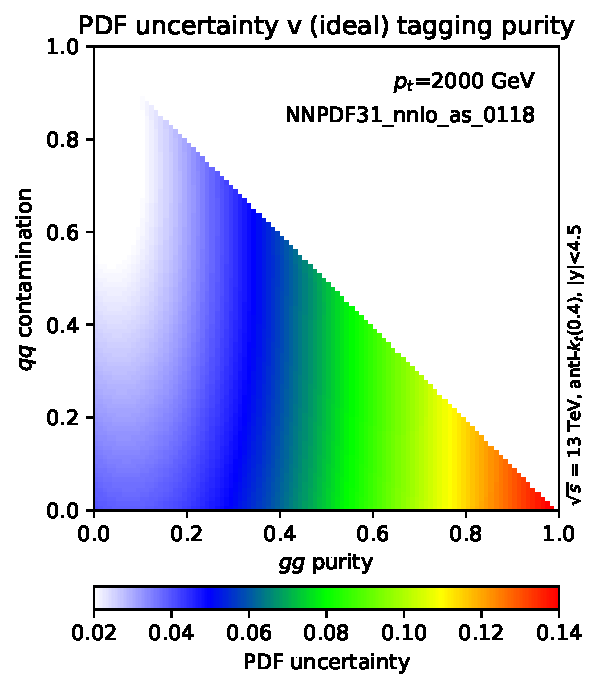
\includegraphics[width=0.42\textwidth, page=1]{figs/performance-plots.pdf} \hfill
\includegraphics[width=0.49\textwidth, page=2]{figs/performance-plots.pdf}
\caption{The plot on the left shows the PDF uncertainty, evaluated using the NNLO set from NNPDF3.1 as a function of $gg$ purity and $qq$ contamination, as defined in the text.
%
The plot on the right shows how the PDF uncertainty compared to experimental systematic and statistical uncertainties, as a function of the $gg$ purity. \sm{Why do we need $\epsilon_g$? Perhaps relabel y-axis.}}
\label{fig:pdf_unc_studies} 
\end{center}
\end{figure}

The next step in our study is to evaluate the current PDF uncertainties, as a function of the final-state flavour composition. 
%
In order to do so, we imagine as a fist step to have at our disposal an idealised tagging procedure that allows us to freely enhance or depress the different partonic components of the final state. We will come back to actual realisations of this tagger later. 
%
In this context, we find useful to define the gluon-gluon ($gg$) purity as
\begin{equation}\label{gg-purity}
gg \, \text{purity}= \frac{\sigma_{gg}}{\sigma_{qq}+\sigma_{qg}+\sigma_{gg}},
\end{equation}
where $\sigma_{ij}$ is the cross section for producing parton $i$ and $j$, evaluated at Born level.  In an analogous way, we can also define the $q q$ contamination is defined analogously, while $q g$ is then fixed by unitarity. Then, for given values $gg$ purity and $qq$ contamination we can evaluate the PDF uncertainty on the cross section.
%
 We decide to perform this estimate using the NNLO PDF set from NNPDF3.1~\cite{Ball:2017nwa} for jets at $2$~TeV.
 %
%The results are shown in Fig.~\ref{fig:pdf_unc_studies}, on the left. 
%
We actually already know from Fig.~\ref{fig:born_studies}, that in the inclusive, i.e.\ untagged, case correspond to $gg$ purity of the order 5\% at $p_t=2$~TeV, while $qq$ and $qg$ makes up roughly 55\% and 40\% of the inclusive sample, respectively. 
%
From the left-hand plot on Fig.~\ref{fig:pdf_unc_studies}, we can then read-off the PDF uncertainty to be of the order of a few percent. This reflects the fact that the quark parton densities are fairly-well constrained in the region of interest. 
As we move to higher values of the $gg$ purity, the less constrained gluon PDFs start to play a more significant role and, as a consequence, the overall uncertainties goes up. For instance, if we were able to devise a tagger that purifies the $gg$ final state to 80\%, we would increase the PDF uncertainty from 2\% to 12\%. 

We can now attempt to assess how go a tagger we should devise in order for the gluon-jet $p_t$ spectrum to be able to constrain the gluon PDF at relatively large $x$. To this purpose we should achieve a situation where the PDF uncertainty is the largest uncertainty, i.e.\ it dominates over the other theoretical and experimental uncertainties. For this feasibility study, we have decided to neglect uncertainties related to the tagging procedure, which can be evaluated, for a given algorithm, using standard scale-variation based, methods. Instead we concentrated on experimental systematic and statistical uncertainties. These uncertainties are shown on the plot in Fig.~\ref{fig:pdf_unc_studies}, on the right, as function fo the $gg$ purity. The experimental systematic uncertainty (in dotted red)  is assumed to be a half of the one reported by the LHC collaboration in 2015~\cite{}, i.e. of the order of 5\%. The statistical uncertainty (in dashed green) correspond to an integrated luminosity of 300 fb$^-1$, i.e.\ roughly the amount of date collected by the end of Run~III of the LHC \sm{Is this true?} 
%
We conclude that the PDF uncertainty becomes the dominant one if the $gg$ purity is above 0.3. Thus, this sets the goal for our tagger.

\begin{figure}
\begin{center}
\includegraphics[width=0.49\textwidth, page=4]{figs/performance-plots.pdf} \hfill
\includegraphics[width=0.49\textwidth, page=5]{figs/performance-plots.pdf}
\caption{}
\label{fig:performance_studies} 
\end{center}
\end{figure}
A variety of techniques to define and discriminate quark-initiated versus gluon-initiated jets has been proposed and studied in the literature. It is customary to express a tagger performance in terms of ROC curves, i.e. plots that exhibits the algorithm ability of identify the signal, i.e. \ its efficiency, versus its mis-tag rate. ROC curves for a handful of quark/gluon taggers are shown in Fig.~\ref{fig:performance_studies}, on the left using a numerical simulation with the Monte Carlo parton shower Pythia~8.230~\cite{}, with the Monash13 tune~\cite{}. The plot shows the signal (gluon) efficiency $\varepsilon_g$ on the horizontal axis and the background (quark) efficiency ($\varepsilon_q$) on the vertical axis. The red-line can be take as the reference and it corresponds to so-called Casimir scaling, and it is related to the universal scaling between the colour factor of the fundamental ($C_F$) and adjoint ($C_A$) representations~\cite{}. 

Because of the different colour factors characterising quark and gluon radiation, gluons tend to radiate more than quarks. Jet shapes~\cite{}, or energy-correlation functions (EFCs)~\cite{} are a probe of such radiation and therefore by selecting jets which exhibit values of the jet shape above a certain threshold, we can enrich our gluon-jet sample. 
% 
Furthermore, jet shapes are fairly-well understood observables and precision-calculations exploiting both fixed-order and resummed perturbation theory are possible, thus systematic reduction of the tagger theoretical uncertainties is, in principle possible. Following the Les Houches studies performed in 2015, the best quark/gluon separation is achieved for the so-called Les Houches ECF: \sm{Do we do $\lambda$ or EFC?} 
\begin{align}\label{LH-EFC}
\text{EFC}^\text{(0.5)}=\sum_{i \in \text{jet}} \left(\frac{p_{ti}}{p_t} \right) \Delta R_i^{1/2}.
\end{align}
The ROC curve for this tagger is shown in green on the left-hand plot of  Fig.~\ref{fig:performance_studies}. We note that despite the fact that jet shapes exhibit Casimir scaling at their lowest order (leading logarithmic accuracy) their discriminating power is increased if higher-order effects are included. For a discussion of such effects, see for instance~\cite{}.

Given the above consideration, it is natural to wonder if it is possible to find substructure tools
which have a different behaviour already at leading-logarithmic
accuracy.
%
The behaviour one would want to obtain is a behaviour like what the particle multiplicity in a jet, or the charged-track multiplicity, typically achieve. In other words, one would like to have a counting observable that, unlike the aforementioned multiplicities exhibits infra-red and collinear safety and therefore can be calculated using perturbation theory. This is requirement is particularly important the context we are discussing as one would have to provide a theoretical calculation for a fit of parton densities. 
%
An observable that ticks all these properties is the Iterated SoftDrop (ISD) multiplicity, which was introduced in Ref.~\cite{}.
%
This algorithm applies the SoftDrop procedure~\cite{} multiple
times, following the hardest branch in
the recursion procedure~\cite{Frye:2017yrw}. This gives a list of
branchings which pass the SoftDrop condition
$(z_1,\theta_1), \dots, (z_n,\theta_n)$. The multiplicity is simply the number of such branchings.
%
It was immediately noticed that for the Iterated SoftDrop multiplicity to be infrared
and collinear safe, one needs either to take a negative value of the SoftDrop angular exponent $\beta$ or impose an explicit cut on the angular separation  $\theta_\text{cut}$.`
%
For we study we employ a variant of the SoftDrop iterated multiplicity which is built setting $\beta=0$ and imposing a minimum relative transverse momentum cut ($k_t=1$~GeV). We name this variant of the Iterated SoftDrop multiplicity, the Les Houches multiplicity ($n_\text{LH}$).
The ROC curve for this tagger is shown in blue on the left-hand plot of  Fig.~\ref{fig:performance_studies}. We notice the gain in the performance, while maintaining full calculability. 

Finally, the ROC curve shown in black corresponds to an extrapolation of the behaviour obtained with a neural-network (NN) architecture exploiting jet topics~\cite{}. This idea originates from techniques employed in text-classification and, as the plot shows, outperforms the Les Houches multiplicity at high gluon efficiencies $\varepsilon_g > 0.5$. Measurements of jet topics have already been performed~\cite{}, however their theoretical understanding is still in its infancy and whether one can perturbatively predict their behaviour is still work in progress.

For each tagger we want to study, we can now pick an efficiency working point $\varepsilon_g$. Then, the corresponding ROC curve will give us the corresponding miss-tag rate $\varepsilon_q$ and with with two inputs we can estimate a realistic $gg$ purity using Eq.~(\ref{gg-purity});
\begin{equation}\label{gg-purity-after-tagging}
gg \, \text{purity}\Big|_\text{after tagging}= \frac{\sigma_{gg} \varepsilon_g^2}{\sigma_{qq}\varepsilon_q^2+\sigma_{qg}\varepsilon_q \varepsilon_g +\sigma_{gg} \varepsilon_g^2},
\end{equation}
and analogously for $qq$ and $qg$. With this information, we are now ready to compile the final plot of this study, which is shown in Fig.~\ref{fig:performance_studies}, on the right. 
This plot is similar in spirit to the right-hand plot of Fig.~\ref{fig:pdf_unc_studies} but now for actual quark/gluon taggers, rather than an idealised one.

As before, we show the different uncertainties: from PDFs ($\delta_\text{PDF}$, solid), statistical uncertainty ($\delta_\text{stat}$, dashed) and systematic one ($\delta_\text{syst}$, dotted). As discussed before, the systematic uncertainty is taken to be constant and equal to 5\%. The statistical uncertainty instead is the square root of the inverse number of the events, and so it  depends on $\varepsilon_g$ (and $\varepsilon_q$). For this, an integrated luminosity of 300~fb$^{-1}$ is assumed. Finally,  the PDF uncertainty of jet cross-section for $p_t>2$~TeV, after tagging is evaluated with NNPDF3.1, as a function of the tagger efficiency. 
%
The plot shows the different uncertainties $\delta_i$ for the taggers mentioned before: a tagger exhibiting simple Casimir scaling (red curves), the Les Houches ECFs (green curves), the Les Houches multiplicity (blue curves) and the neural-network tagger (black curves). The systematic uncertainty is assumed to be the same for each tagger. 
%
The plot shows that for jets with transverse momentum above 2~TeV a pure Casimir-scaling tagger or a ECF-based tagger are never good enough to enrich the final-state gluon content such that $\delta_\text{PDF}> \delta_\text{syst}, \delta_{stat}$.
%
Instead, if we pick $\epsilon_g\simeq 0.5$ the $n_\text{LH}$ tagger and the NN one do provide $\delta_\text{PDF}$ which are comparable, if not definitely bigger, then statistical and systematic uncertainties. This is definitely more marked for the NN tagger but, as mentioned before, it is currently unclear how to perform perturbative calculations for this. On the other hand, the jet transverse momentum distribution with a cut on $n_\text{LH}$ is well-defined and calculable in perturbation theory. 
